

\begin{frame}{Qu'est-ce qu'une transaction\,?}

\begin{defblock}{Définition}
Une transaction est une séquence d'opérations de \alert{lecture} ou d'\alert{écriture}, 
se terminant par \sqlkw{commit} ou \sqlkw{rollback}.
\end{defblock}

\vfill

\begin{redbullet}
  \item Le \sqlkw{commit}  \alert{valide} \textit{toutes} les mises à jour.
  \item Le \sqlkw{rollback} \alert{annule} \textit{toutes} les mises à jour.
\end{redbullet}
\vfill

\begin{block}{\alert{Propriétés}\,: atomicité et durabilité}
\begin{redbullet}
  \item Les opérations d'une transaction sont solidaires: elles sont toutes validées, ou pas du tout.
   \item Un \sqlkw{commit} exécuté  est \alert{définitif}, même si une panne survient
\end{redbullet}
\end{block}
\end{frame}

\begin{frame}{Exemple\,: réservation de billets}

\begin{redbullet}

  \item Des clients \texttt{Client (id, nom, nbBillets)}
  \item Des vols \texttt{Vol(id, intitulé, capacité, nbRéservations)} 
\end{redbullet}

\vfill

Une réservation est cohérente si les deux opérations sont \alert{solidaires}\,:

\begin{redbullet}

  \item La MAJ de  \texttt{Client} pour affecter le nombre de billets achetés
  \item La MAJ de \texttt{Vol} pour affecter le nombre de réservations
\end{redbullet}

\vfill
\begin{block}{\alert{Propriété}\,: la cohérence}
Cette base est \alert{cohérente} si le nombre de billets des clients
est égal à au nombre de réservations du vol.
\end{block}
\end{frame}


\begin{frame}[fragile]{Un programme qui engendre des transactions}

\begin{minted}[frame=leftline,
               baselinestretch=.8,
               fontsize=\small,
               framesep=2mm]{sql}
    -- On recherche le vol pour vérifier les places libres
    select * into vol from Vol where id=v_idVol
    -- On recherche le client pour vérifier son identité
    select * into client from Client where id=v_idClient;
    
    -- Calcul des nouvelles valeurs
    calculBillets = client.nbBillets + nbBillets
    calculRésas = vol.réservations + nbBillets
    
    -- On modifie
    update Client set nbBillets=calculBillets 
         where id=v_idClient;
    update Vol set réservations = calculRésas  
         where id=v_idVol;
    commit;
 \end{minted}

\vfill

Trois phases, typiques\,: lectures, calcul, mises à jour, \sqlkw{commit}
\end{frame}

\begin{frame}{Exécutions concurrentes}

Quand plusieurs réservations s'effectuent simultanément, 
les transactions engendrées sont \alert{en concurrence}.

\vfill

\begin{center}
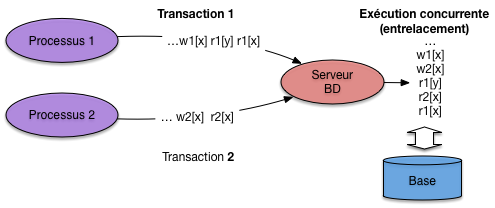
\includegraphics[width=8cm]{../../figures/exec-concurrentes}
\end{center}

\vfill


\begin{block}{\alert{Propriété}\,: l'isolation}
Chaque transaction doit se comporter comme si elle était
la seule à s'exécuter. 
\end{block}

\end{frame}

\begin{frame}{Résumé\,: propriétés des transactions}

Transaction = séquence de lecture et mises à jour 
 se terminant par \sqlkw{commit} ou \sqlkw{rollback}

\vfill

Le SGBD 
garantit des propriétés dites ACID.

\begin{redbullet}

  \item  \alert{Atomicité}. Validation complète, ou annulation complète
  
  \item  \alert{Cohérence}. Passage d'un état cohérent à un autre état cohérent.
  
  \item \alert{Isolation}. Une transaction s'exécute comme si elle était seule.
  
   \item \alert{Durabilité}. Un  \sqlkw{commit} qui s'exécute est  définitif.
\end{redbullet}

\vfill

\begin{block}{\alert{En pratique}}
Plusieurs niveaux d'isolation\,: compromis performance/cohérence.
\end{block}
\end{frame}
